\chapter{Volatility scaling across network topologies}
\label{chap:results}

With the rescaled integrator of Chapter~\ref{chap:rescaling} we can hold the GLV
system exactly at its cooperative critical point and read off long, scale-spanning
transients that an explicit solver could never resolve. This chapter uses that tool
to ask the question posed in the introduction: does a static GLV network tuned to
$\mu_c$ reproduce the two empirical firm-growth regularities---the slow
size--volatility decay $\sigma(S)\sim S^{-\beta}$ with $\beta\approx0.15$--$0.20$, and
the fat-tailed, non-Gaussian growth-rate distribution---and how do the answers depend
on the topology of the inter-firm network?

We sweep three degree distributions at fixed mean degree---a \emph{regular} graph
($k=C$ for all nodes, no degree variance), an \emph{exponential} configuration model
($k\sim\mathrm{Exp}(C)$), and a \emph{power-law} graph ($p(k)\propto k^{-\alpha}$ with
$\alpha=2.5$ held fixed and the lower cutoff set so the mean degree tracks $C$)---and
a connectivity range $C\in\{5,10,20,40\}$. Throughout we fix $N=1000$ and disorder
$\sigma=0.2$, place the system at the per-topology critical point $\mu_c$ located with
the shape-scalar estimator of Section~\ref{sec:estimator-c}, and average each
observable over $40$ independent graph realizations.

\section{Observables}
\label{sec:observables}

We treat each node as a firm and its abundance as the firm's size. To mirror how the
empirical exponents are measured we normalize sizes within each cross-section: writing
$\tilde{S}_{iy}$ for the raw abundance of firm $i$ in year $y$, the normalized size is
\begin{equation}
    S_{iy} = N\,\frac{\tilde{S}_{iy}}{\sum_j \tilde{S}_{jy}},
    \label{eq:size-norm}
\end{equation}
so the cross-sectional mean size is $1$ in every year and the common-mode growth of
the total abundance---which at $\mu_c$ is precisely the diverging envelope $M(t)$---is
divided out, leaving only the \emph{relative} reshuffling of firms. This is the
cross-sectional normalization of \citet{moran2024}. The (log) growth rate and its
time-averaged volatility are
\begin{equation}
    g_{iy} = \ln\frac{S_{i,y+1}}{S_{iy}}, \qquad
    \sigma_i = \sqrt{\tfrac{\pi}{2}}\,\frac{1}{T_i}\sum_y \bigl|\,g_{iy}-\bar{g}_i\,\bigr|,
    \label{eq:vol-mad}
\end{equation}
where the mean-absolute-deviation estimator (rescaled by $\sqrt{\pi/2}$, the
Gaussian-consistent factor) is used in place of the standard deviation for robustness
against the fat tails of $g$. Physical-time trajectories $x(t)=M(t)\,y(t)$ are
reconstructed from a rescaled run and sampled on a uniform grid of $100$ ``years''
between $t=0$ and the (finite) blow-up time $t^\ast$; Figure~\ref{fig:res-traj} shows a
sample. At $\mu_c$ with modest disorder the relative sizes disperse only mildly and
never collapse---no firm goes extinct---which is what makes the size--variance fit
below well-conditioned over the whole population rather than a surviving subset.

\begin{figure}[htbp]
    \centering
    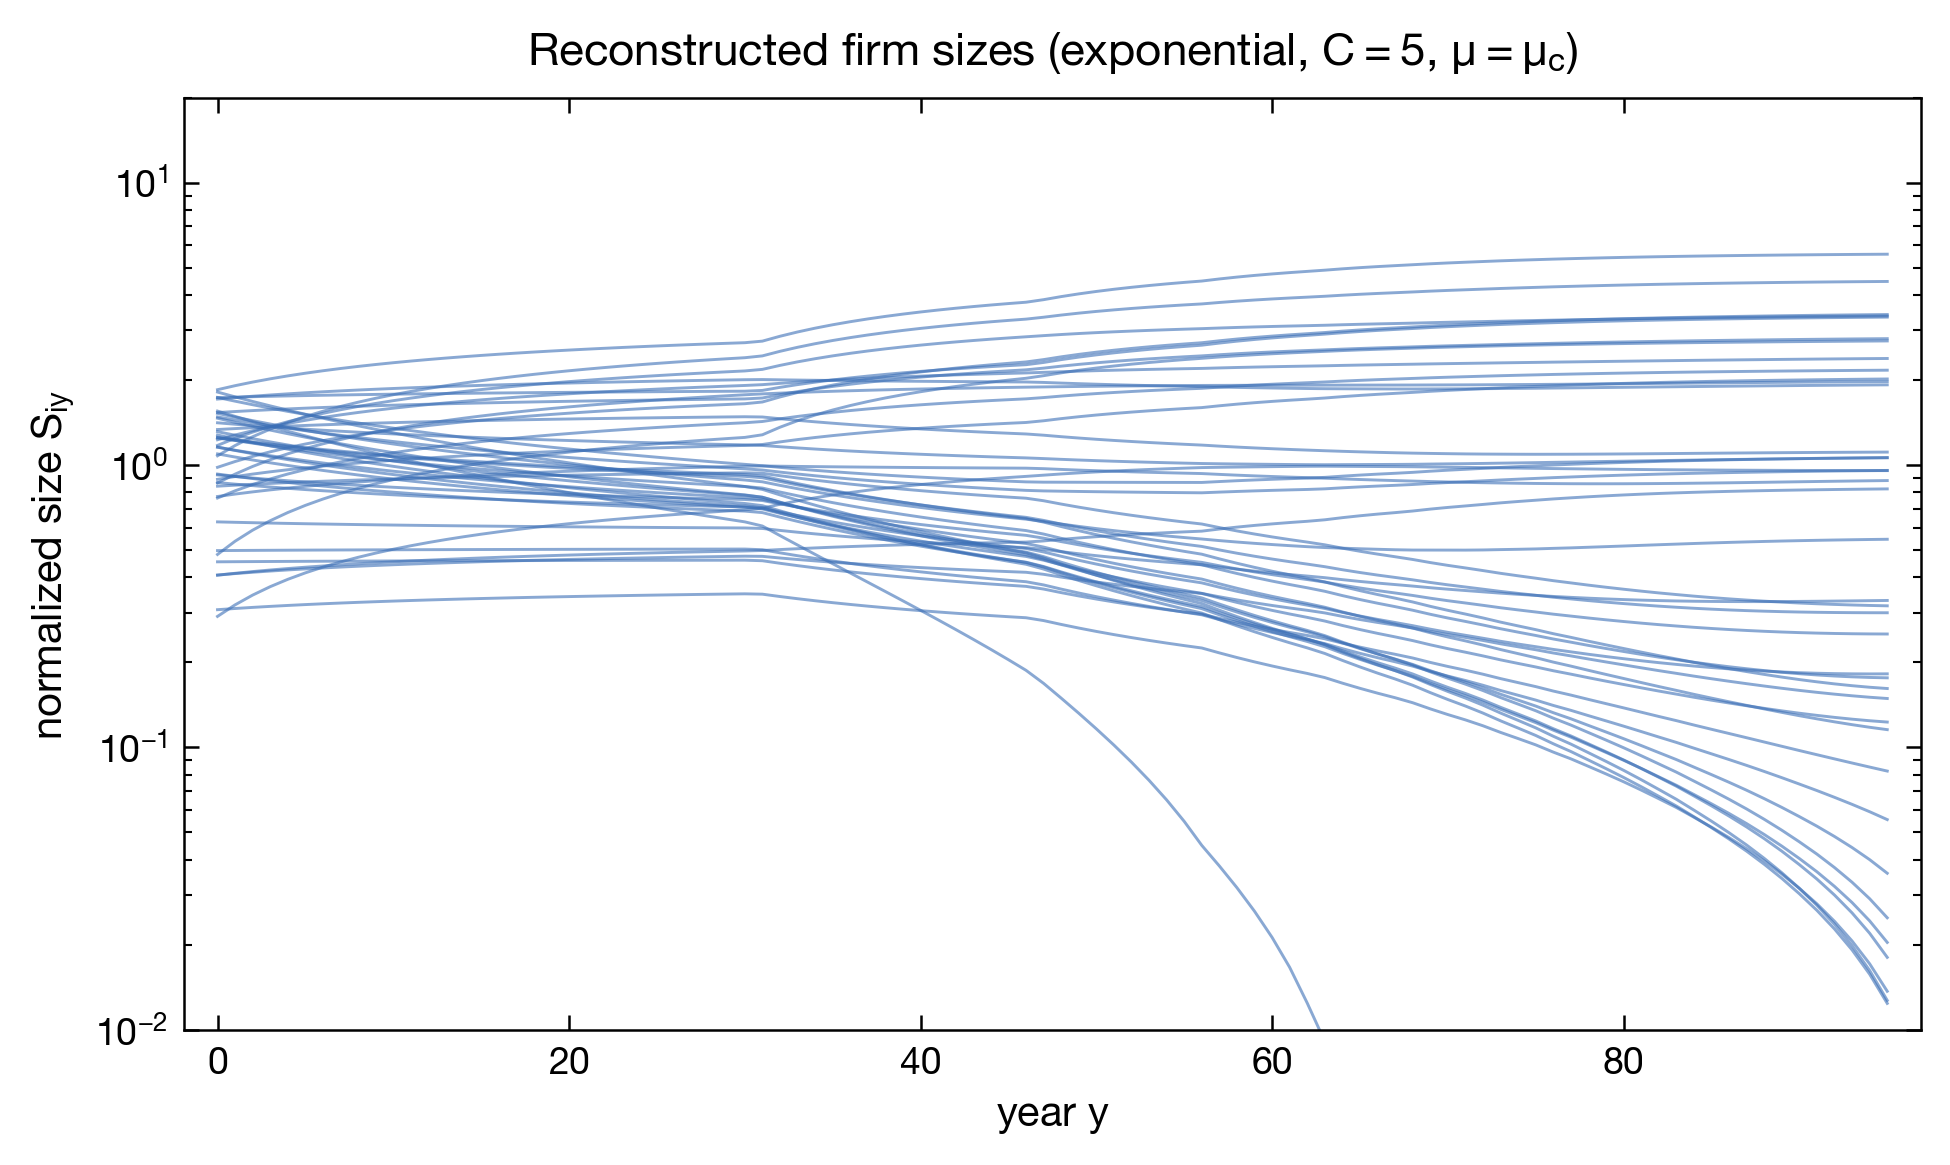
\includegraphics[width=0.85\linewidth]{results_trajectory.png}
    \caption{Reconstructed normalized firm sizes $S_{iy}$ for a sample of $40$ firms on
    an exponential graph at $C=5$, $\mu=\mu_c$. Sizes spread over roughly two decades
    and persist---the mild, non-decaying dispersion characteristic of the critical
    transient. (The final few reconstructed years are dropped, where the large
    envelope $M$ degrades the $x=My$ reconstruction as discussed in
    Section~\ref{sec:numerical-integration}.)}
    \label{fig:res-traj}
\end{figure}

\section{The critical point as the selected operating point}
\label{sec:operating-point}

The choice to sit exactly at $\mu_c$ is not a free parameter but is forced by the
dynamics. The cooperative coupling $\mu$ selects between three qualitatively
different regimes. For $\mu<\mu_c$ the interior equilibrium is stable: every firm
relaxes to a fixed size, all growth rates decay to zero, and the growth-rate
distribution collapses to a degenerate spike at the origin---there is no economy
to speak of, and no nondegenerate distribution to compare against the data. For
$\mu>\mu_c$ the system still grows without bound, but the right tail of the
growth-rate distribution becomes too thin: the large-growth episodes that are the
defining heavy-tailed feature of the empirical distribution are suppressed, and
the tail decays too fast to match the data. Only at the critical point $\mu_c$,
the boundary between the two, does the system grow without bound while retaining a
fat tail---the slowest blow-up sustains the longest-lived transient and the widest
cross-sectional reshuffling of relative sizes, which is precisely what produces
the sharply peaked, heavy-tailed growth-rate distribution the data demand.

Criticality is therefore selected by one of the two empirical facts we are trying
to reproduce. The growth-rate distribution is realistic only at $\mu_c$, which
fixes the operating point with no remaining freedom. The size--variance exponent
$\beta$ measured there is, in consequence, a \emph{parameter-free prediction}:
once the distribution constraint has pinned $\mu$ to $\mu_c$, nothing is left to
tune, and $\beta$ is simply whatever the critical dynamics deliver. This is what
makes the comparison with the empirical exponent meaningful---it is a genuine
prediction of the model rather than the result of a fit.

\section{The size--variance relation}
\label{sec:sizevar-baseline}

We pool the per-firm pairs $(\bar{S}_i,\sigma_i)$ over all realizations, bin them into
equal-count size bins, and fit $\log\sigma_i = -\beta\,\log\bar{S}_i + \text{const}$.
Figure~\ref{fig:res-sizevar-baseline} shows the baseline case (exponential graph,
$C=5$): the volatility does fall with size as a power law, with
\begin{equation}
    \beta = 0.51 \pm 0.10 .
\end{equation}
This already sits between the two reference values: it is below the naive
$\beta=1/2$ expected for a firm built from independent sub-units, confirming that the
inter-firm couplings generate genuine size-dependent correlations and partially defeat
diversification---but it is well above the empirical $\beta\approx0.15$--$0.20$. The
inter-firm GLV mechanism therefore produces an anomalous exponent in the right
direction, but not nearly anomalous enough.

\begin{figure}[htbp]
    \centering
    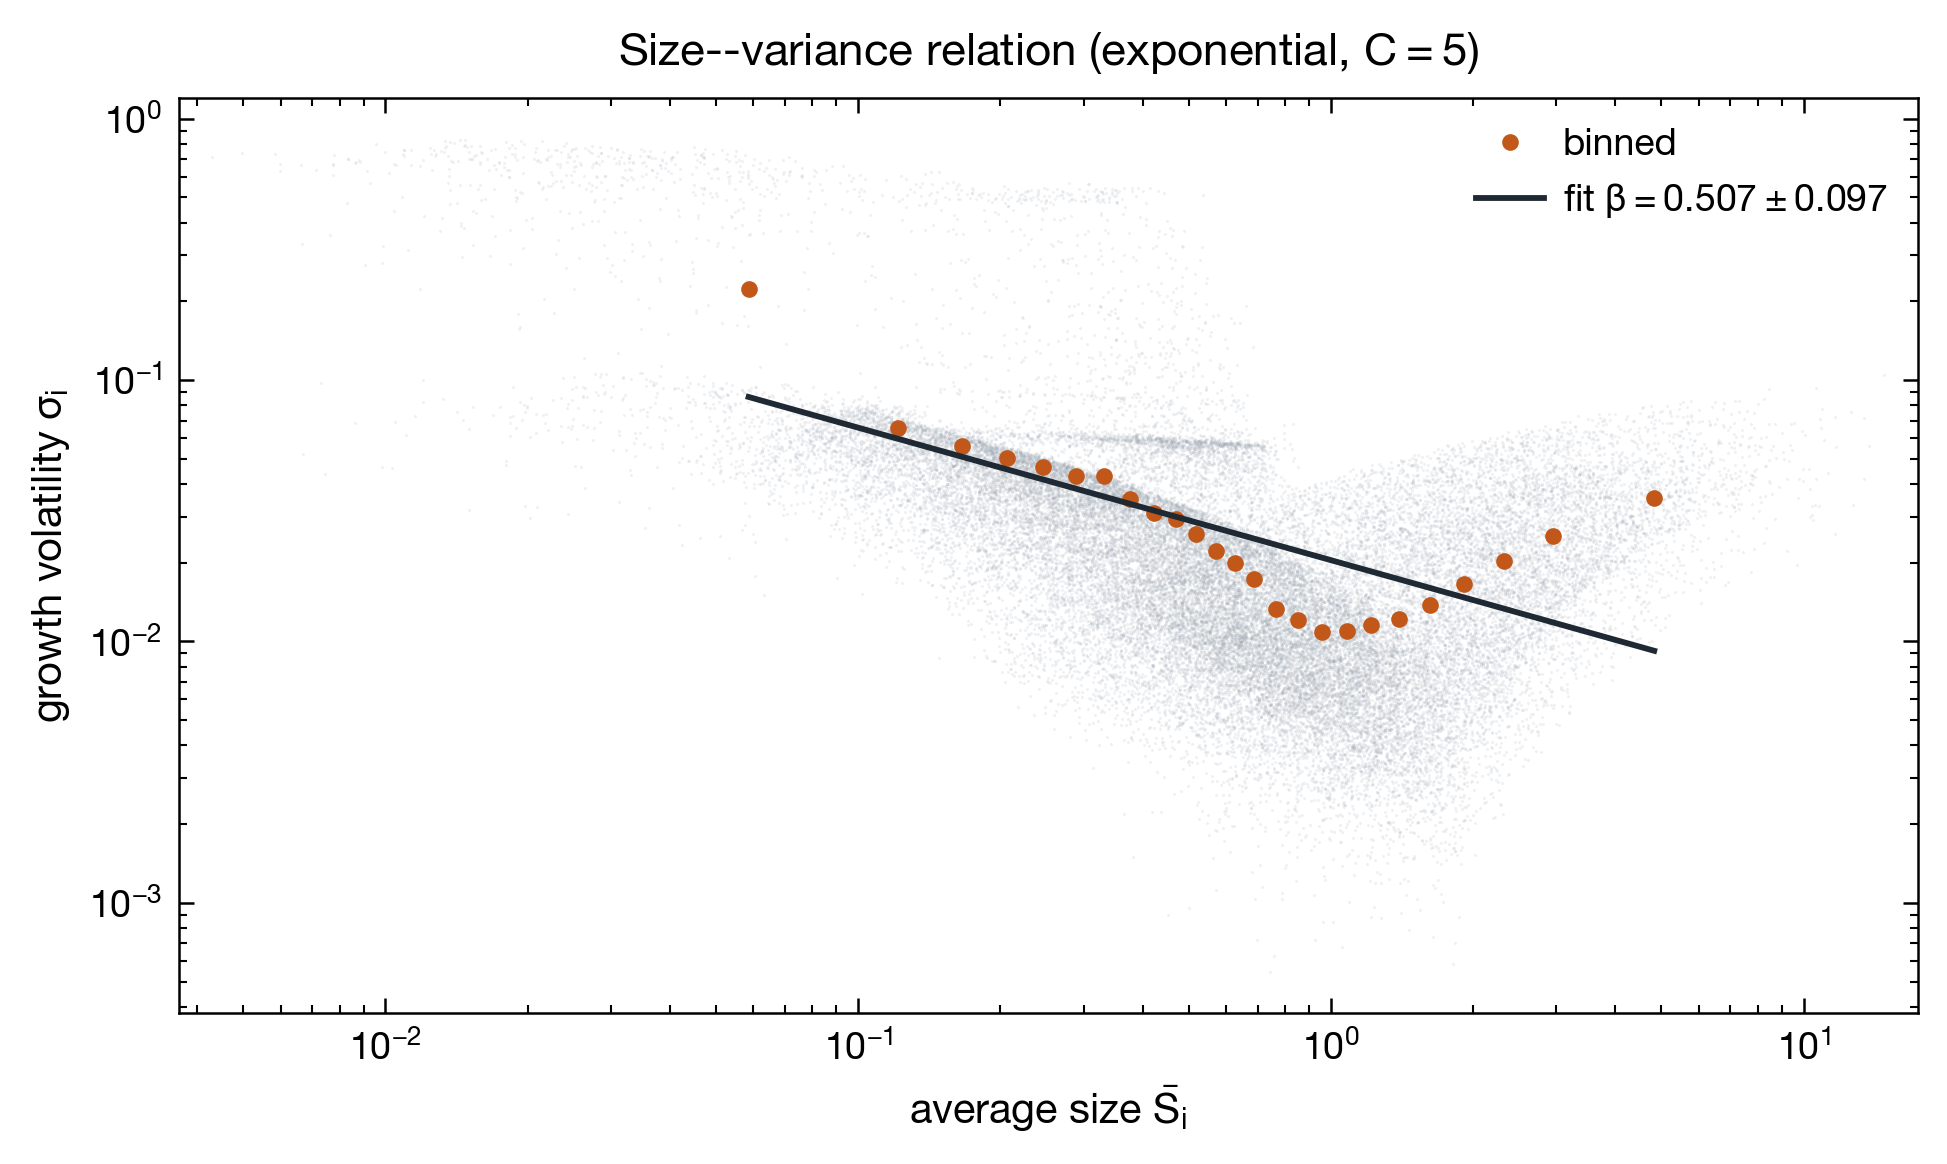
\includegraphics[width=0.85\linewidth]{results_sizevar_baseline.png}
    \caption{Size--variance relation for the exponential graph at $C=5$, $\mu=\mu_c$.
    Faint points are individual firms pooled over $40$ realizations; orange markers are
    equal-count bin averages; the line is the power-law fit $\sigma_i\sim
    \bar{S}_i^{-\beta}$ with $\beta=0.51\pm0.10$.}
    \label{fig:res-sizevar-baseline}
\end{figure}

\section{Dependence on topology}
\label{sec:topology}

Holding $C=5$ fixed and varying only the degree distribution
(Figure~\ref{fig:res-sizevar-topology}) shows that the exponent \emph{grows} with
degree heterogeneity: $\beta=0.29$ for the regular graph, $0.51$ for the exponential,
and $0.86$ for the power-law. This is the opposite of what the granular intuition
might suggest---there a heavier-tailed structure produces a \emph{slower} decay
(smaller $\beta$). Here the heavy-tailed degree distribution instead makes the
volatility fall \emph{faster} with size: the well-connected hubs, which carry the
largest abundances, average over many neighbours and so fluctuate proportionally less,
steepening the relation. The same heterogeneity also lowers the critical point, since
$\mu_c$ is governed by $\langle g^2\rangle$ with $g=k/C$ (Table~\ref{tab:res-summary}):
$\mu_c\approx0.99$ (regular), $0.49$ (exponential), $0.26$ (power-law).

\begin{figure}[htbp]
    \centering
    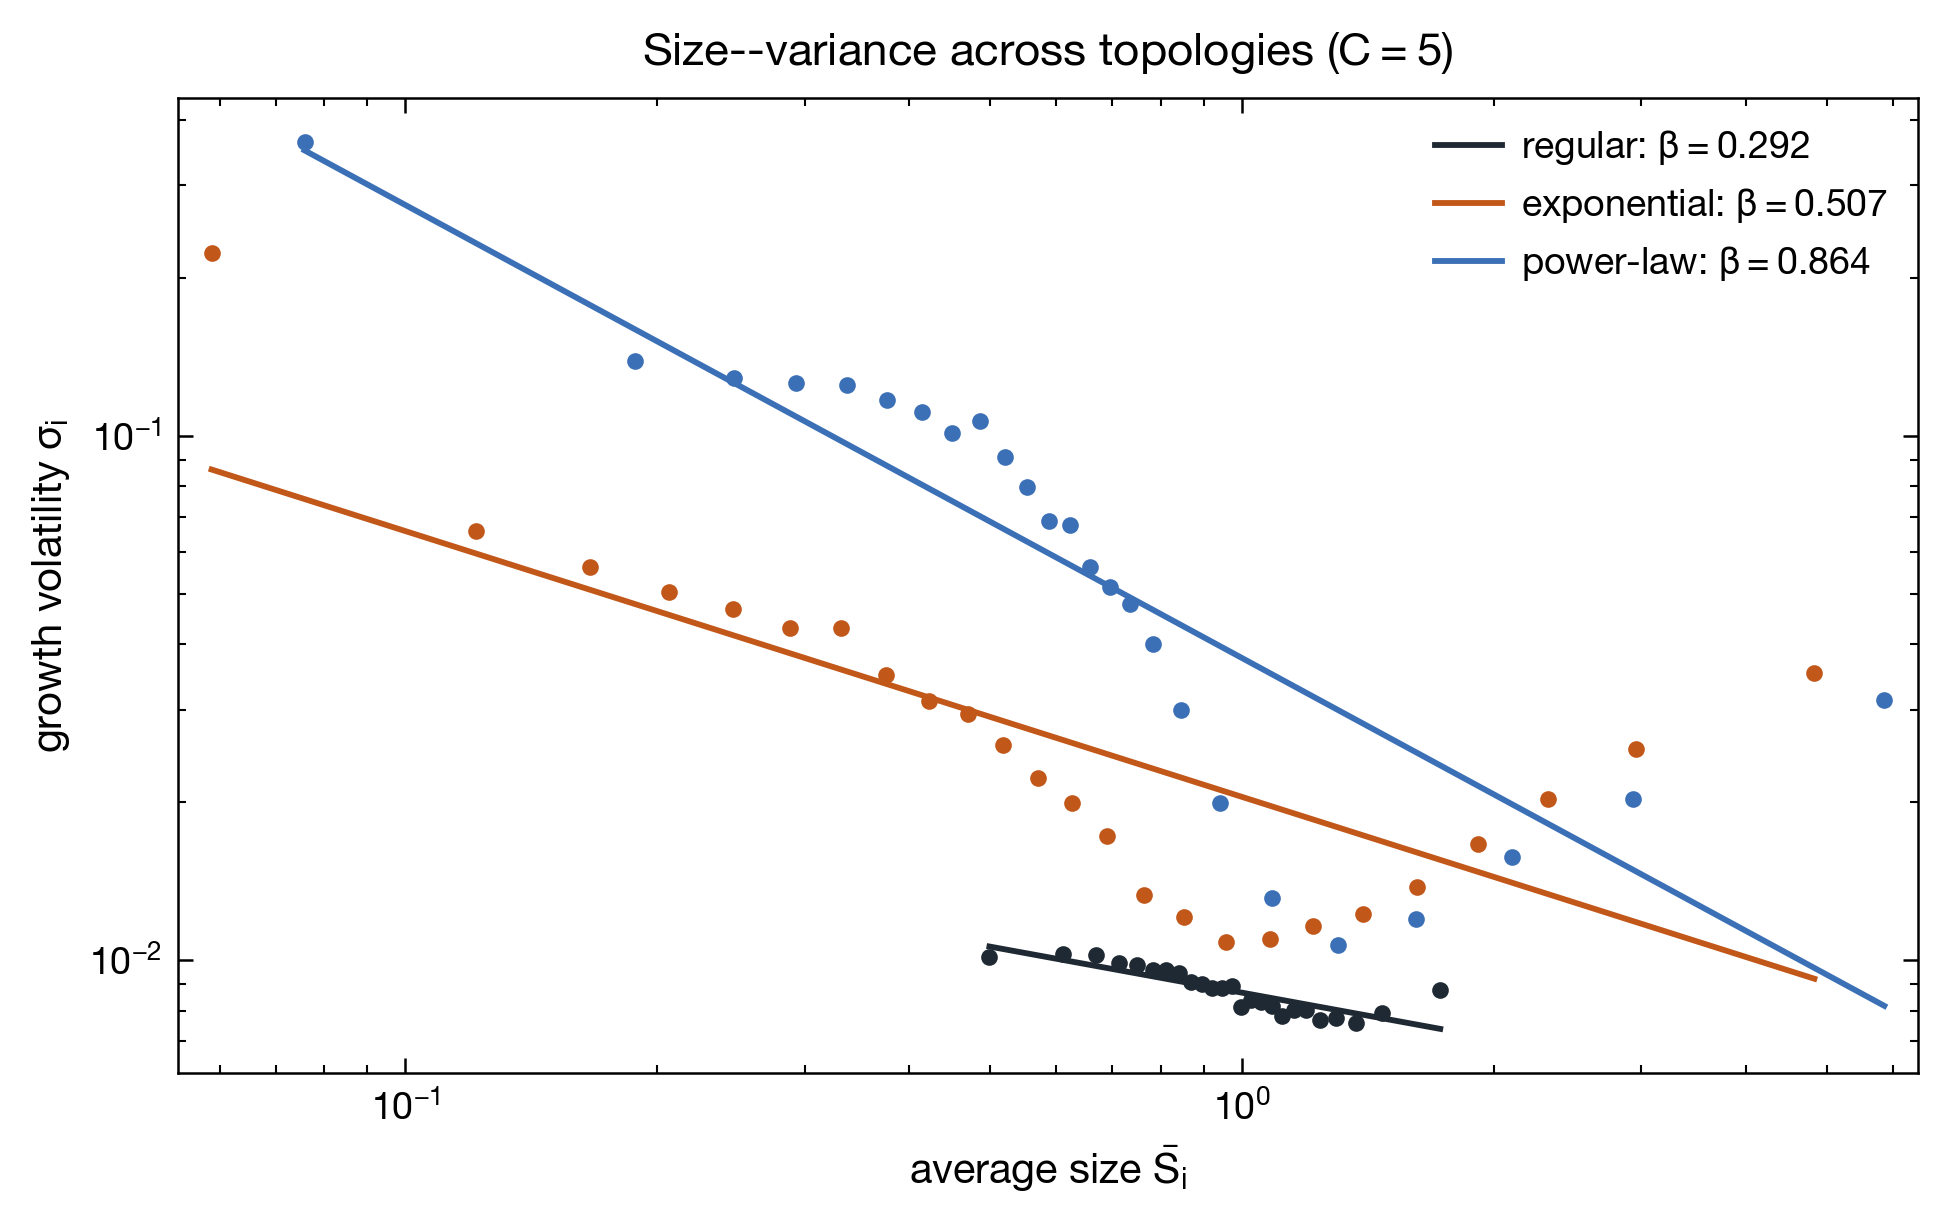
\includegraphics[width=0.85\linewidth]{results_sizevar_topology.png}
    \caption{Size--variance relation across the three topologies at $C=5$, $\mu=\mu_c$
    (equal-count bin averages and power-law fits). The exponent grows with degree
    heterogeneity: regular $<$ exponential $<$ power-law.}
    \label{fig:res-sizevar-topology}
\end{figure}

\section{Dependence on connectivity}
\label{sec:connectivity}

Sweeping the mean degree $C$ (Figure~\ref{fig:res-beta-C}) shows that $\beta$ also
\emph{increases} with connectivity for every topology---most cleanly for the regular
and exponential graphs, where it climbs from $\approx0.3$--$0.5$ at $C=5$ toward
$\approx0.6$--$0.8$ at $C=40$; the power-law curve is noisier but stays highest
throughout. Denser networks give each firm more neighbours to average against, which
again steepens the size--volatility decay. The trend is unfavourable for matching the
data: the empirical band $0.15$--$0.20$ (shaded) lies below \emph{all} measured
points, and increasing connectivity moves the model away from it rather than toward it.

\begin{figure}[htbp]
    \centering
    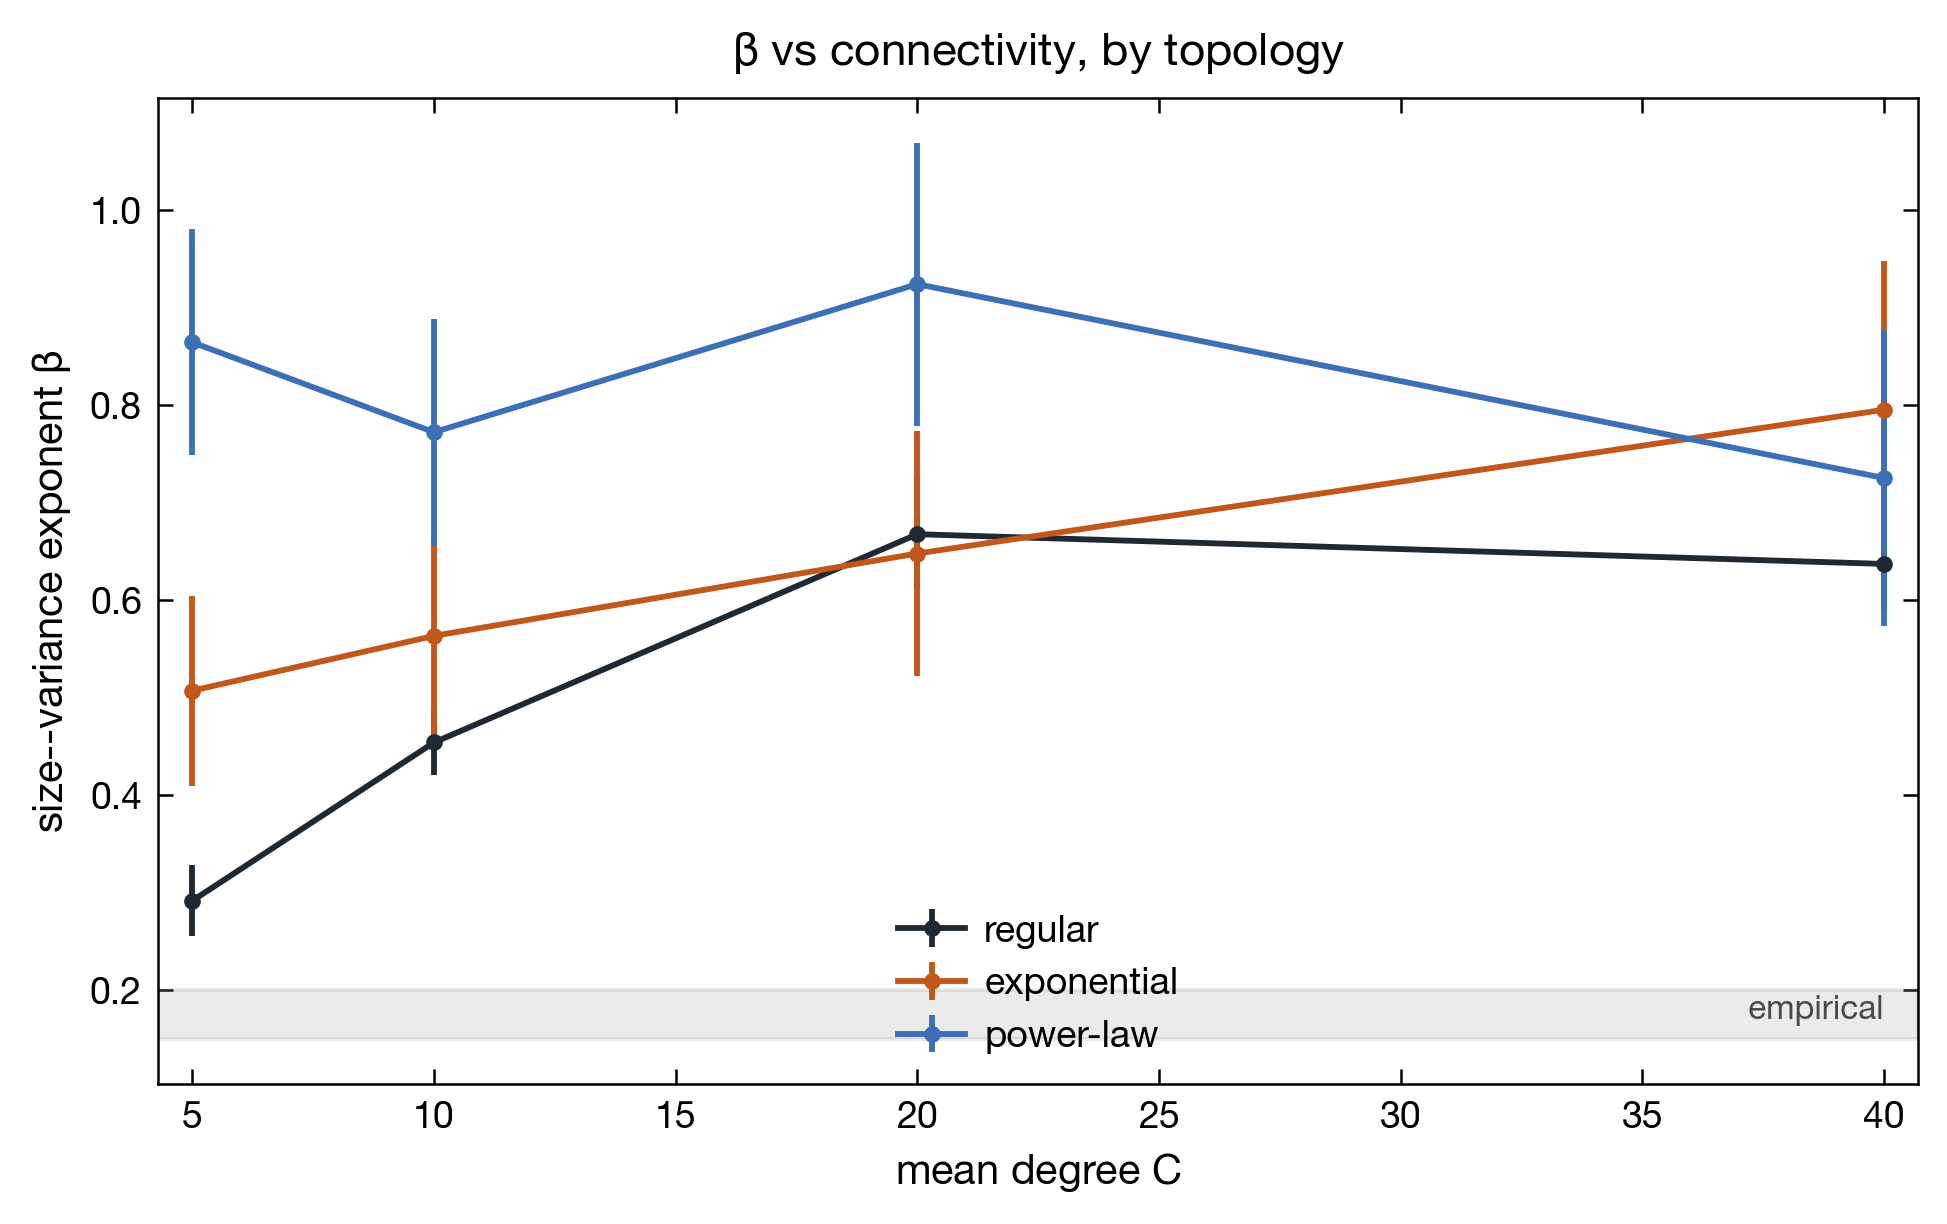
\includegraphics[width=0.85\linewidth]{results_beta_vs_C.png}
    \caption{Size--variance exponent $\beta$ versus mean degree $C$, by topology (mean
    $\pm$ fit standard error over $40$ realizations). The empirical range
    $0.15$--$0.20$ is shaded; every measured $\beta$ lies above it, and $\beta$ rises
    with $C$.}
    \label{fig:res-beta-C}
\end{figure}

That the fit is read off the full population, not a surviving remnant, is confirmed by
Figure~\ref{fig:res-survival}: the fraction of firms with $\bar{S}_i>10^{-2}$ stays
above $0.994$ across every topology and connectivity. Extinction plays no role at
$\mu_c$ with $\sigma=0.2$; the size dispersion is generated entirely by the
interactions, not by a collapse onto a few survivors. The critical point itself drifts
upward with $C$ for the heterogeneous graphs (Table~\ref{tab:res-summary})---the
finite-size effect analysed in Section~\ref{sec:muc-statistics}, where raising $C$ at
fixed $N$ erodes the locally tree-like structure the mean field assumes.

\begin{figure}[htbp]
    \centering
    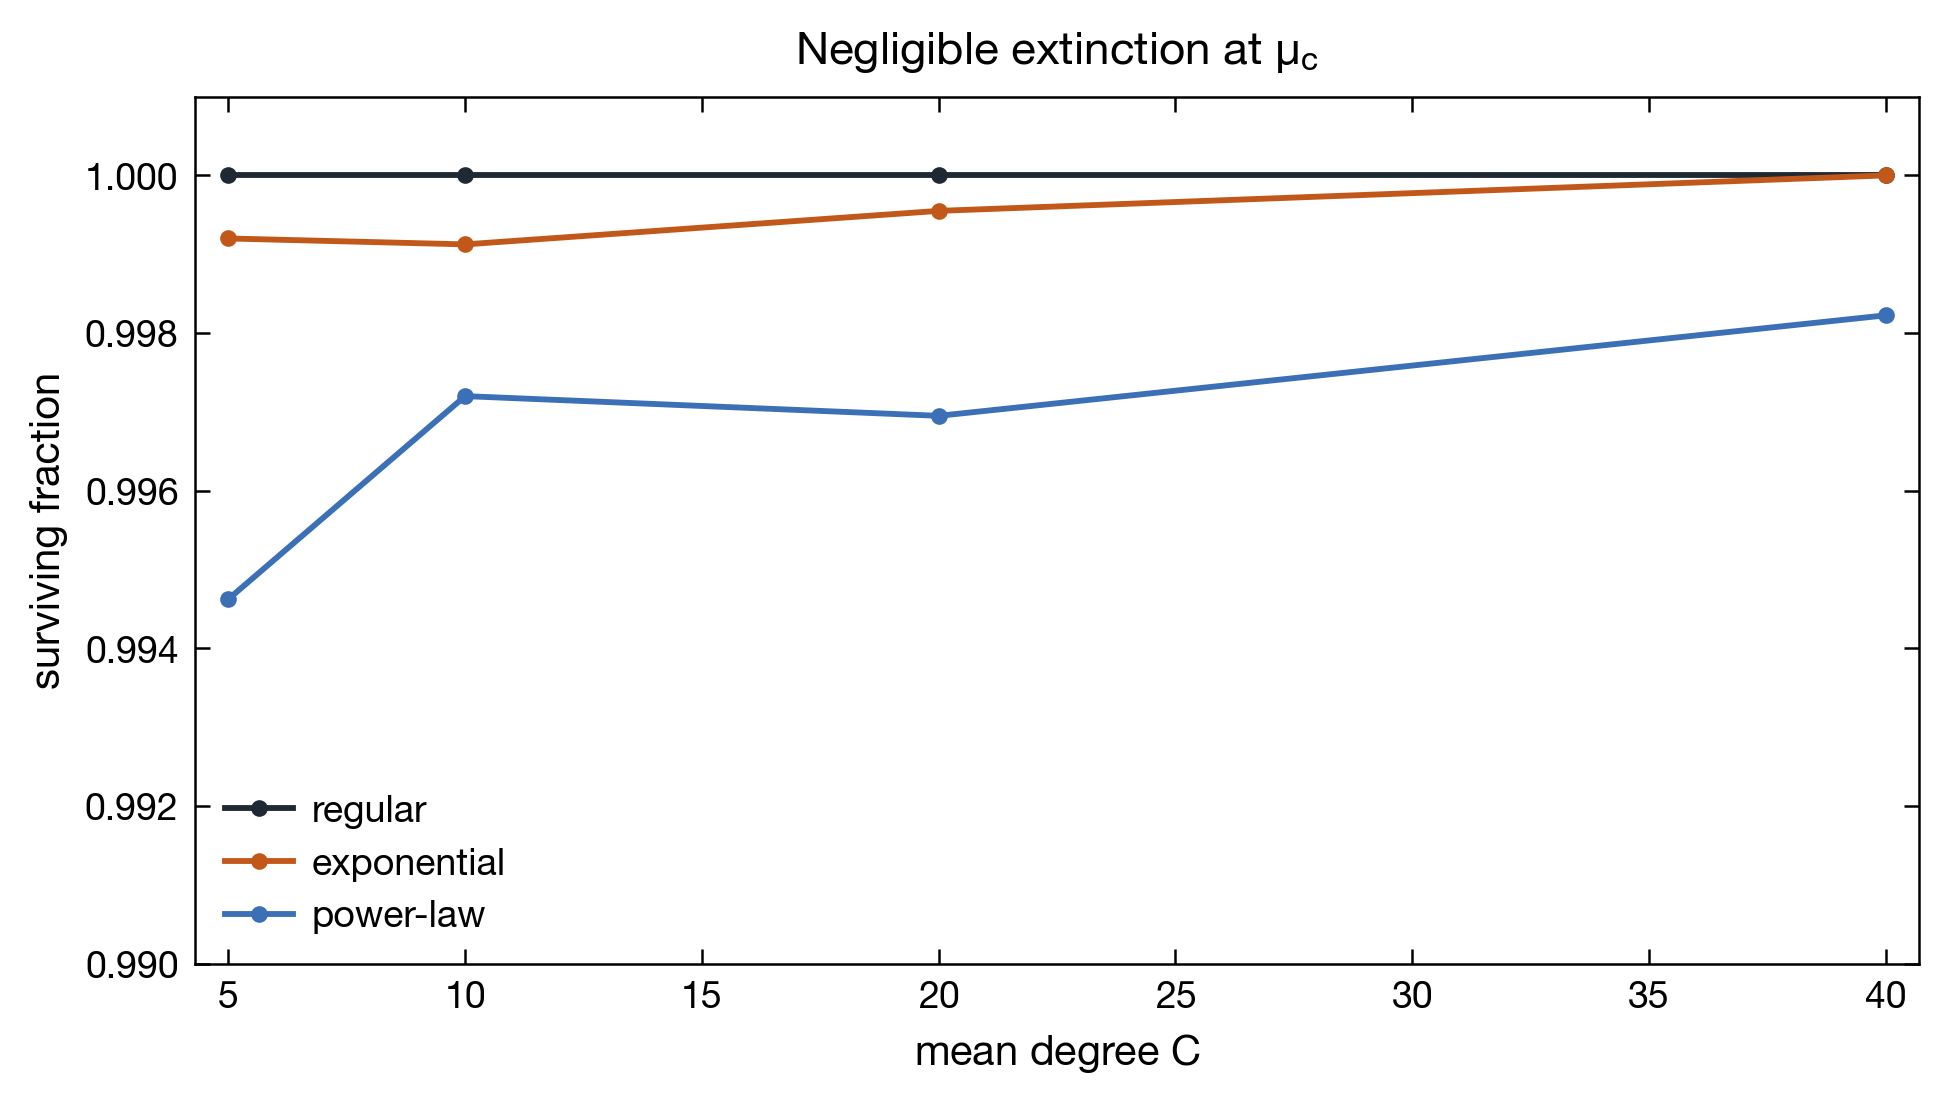
\includegraphics[width=0.8\linewidth]{results_survival.png}
    \caption{Surviving fraction (firms with $\bar{S}_i>10^{-2}$) versus $C$. It remains
    essentially $1$ everywhere, so the size--variance fit uses the whole population.}
    \label{fig:res-survival}
\end{figure}

\begin{table}[htbp]
    \centering
    \begin{tabular}{llcccc}
        \hline
        & $C$ & $5$ & $10$ & $20$ & $40$ \\
        \hline
        \multirow{2}{*}{regular}
          & $\beta$   & $0.29\pm0.04$ & $0.45\pm0.03$ & $0.67\pm0.06$ & $0.64\pm0.05$ \\
          & $\mu_c$   & $0.99$ & $1.00$ & $1.01$ & $1.02$ \\
        \multirow{2}{*}{exponential}
          & $\beta$   & $0.51\pm0.10$ & $0.56\pm0.11$ & $0.65\pm0.13$ & $0.80\pm0.15$ \\
          & $\mu_c$   & $0.49$ & $0.52$ & $0.54$ & $0.60$ \\
        \multirow{2}{*}{power-law}
          & $\beta$   & $0.86\pm0.12$ & $0.77\pm0.12$ & $0.92\pm0.15$ & $0.73\pm0.15$ \\
          & $\mu_c$   & $0.26$ & $0.44$ & $0.46$ & $0.61$ \\
        \hline
    \end{tabular}
    \caption{Size--variance exponent $\beta$ (fit $\pm$ standard error) and located
    critical point $\mu_c$ for each topology and mean degree $C$, at $N=1000$,
    $\sigma=0.2$. Degree heterogeneity lowers $\mu_c$ and raises $\beta$; connectivity
    raises $\beta$.}
    \label{tab:res-summary}
\end{table}

\section{The growth-rate distribution}
\label{sec:growthdist}

The second empirical fact is the shape of the growth-rate distribution, which in the
data is sharply peaked and fat-tailed rather than Gaussian. Here the model does
better. Figure~\ref{fig:res-growthdist} overlays the pooled growth rates for the three
topologies, standardized by their own scale, against a Laplace reference. All three are
strongly non-Gaussian---peaked at zero with roughly exponential (tent-shaped) flanks
spanning several decades---reproducing the qualitative form reported by
\citet{stanley1996} and \citet{amaral1997}. The regular graph is the most heavy-tailed,
tracking the Laplace line out to $\pm6$ standard deviations, while the heterogeneous
graphs are more peaked in the centre with somewhat lighter, mildly asymmetric tails.
So the fat-tailed shape emerges endogenously from the critical dynamics on any of the
topologies, even though the size--variance exponent does not match.

\begin{figure}[htbp]
    \centering
    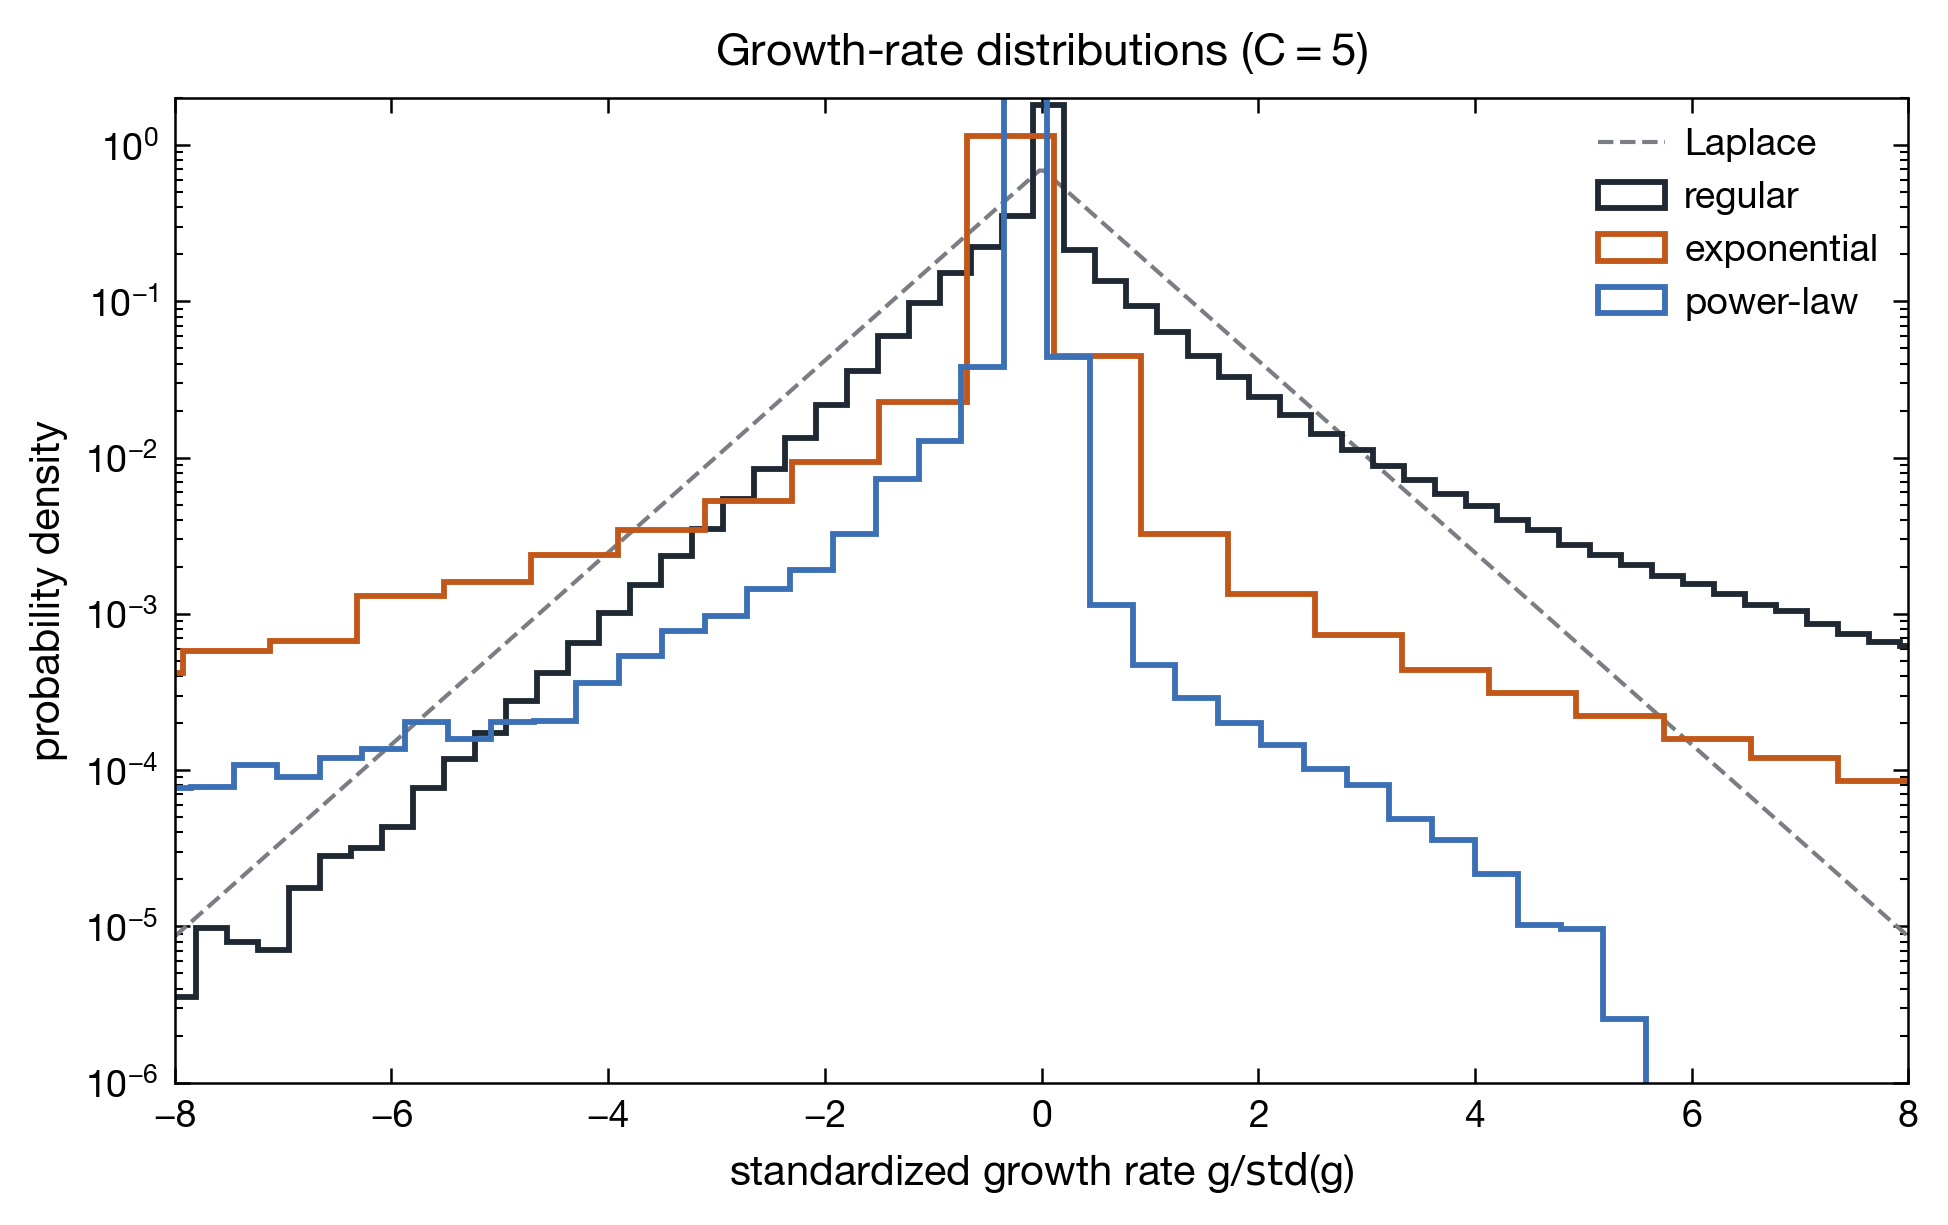
\includegraphics[width=0.85\linewidth]{results_growthdist.png}
    \caption{Growth-rate distributions at $C=5$, standardized by their own standard
    deviation, for the three topologies, with a Laplace reference (dashed). All are
    sharply peaked and fat-tailed---clearly non-Gaussian---with the regular graph the
    most Laplace-like.}
    \label{fig:res-growthdist}
\end{figure}

\section{Discussion}
\label{sec:results-discussion}

Pulling the two measurements together gives a split verdict on the question of the
introduction. A static GLV network tuned to its critical point \emph{does} reproduce
the non-Gaussian, fat-tailed shape of the growth-rate distribution, and it \emph{does}
push the size--variance exponent below the naive $\beta=1/2$, confirming that
inter-firm couplings create genuine size-dependent correlations that interfere with
diversification. But it does \emph{not} reproduce the empirically slow decay: every
measured $\beta$ lies in the range $0.3$--$0.9$, well above the observed
$0.15$--$0.20$, and the exponent moves the \emph{wrong way} under both structural
knobs---it grows with degree heterogeneity and with connectivity, because better-mixed
and better-connected firms average over more neighbours and fluctuate relatively less.
The granular mechanism of \citet{moran2024} and \citet{wyartbouchaud2003}, where a
heavy-tailed \emph{size} composition makes diversification fail, therefore remains
necessary: topological criticality alone, with the homogeneous self-regulation used
here, supplies the heavy tails but not the anomalously slow size--variance scaling.
The natural next step---moving off-criticality, weakening the self-regulation, or
correlating a firm's intrinsic volatility with its connectivity---is sketched in
Chapter~\ref{chap:conclusion}.
